\chapter{Distribution System Design} \label{chapDistDesign}

This chapter deals with the design of a distribution network (or the re-design of an existing supply chain). Controlling a supply chain focuses on the description of the processes and the day-by-day planning; on the other hand, the design of a network profoundly modify the distribution strategy for many actors of the chain. The design activities are classified depending on the decision patterns (see section \ref{secDecisionPatternsDistribution}) involved into:

\begin{enumerate}
    \item Location-allocation problem, i.e. clustering points of demand of the network into groups without exceeding the capacity of the resources assigned to each group;
    \item Network topology design, i.e. the definition of service routes within each cluster;
    \item Route frequency design, i. e. defining the frequency of service for each node of the network;
    \item Service time windows design, i.e. defining the time interval when each node of the network should be served;
    \item Shipping priority definition, i.e. identify dispatching rules for HUs.

\end{enumerate}

These problems can be seen in the perspective of a hierarchical procedure to design a distribution network from scratch. First of all, for each terminal $j$ of the network, it is necessary to investigate:

\begin{enumerate}
    \item its position (i.e. the longitude, and the latitude);
    \item its demand;
    \item its serving infrastructure is identified (e.g. road, rail, water).
\end{enumerate}

Then, the location-allocation problem LAP (1) identifies the number of resources, their capacity, and their location to satisfy the demand of the nodes. The design of the routeing topology (2) assign each terminal $j$ to a route e travelled by a vehicle $v$ connecting the terminal to one of the resources (e.g. production plant or storage system) identified by the LAP. The design of the route frequency (3) matches the demand of the terminal, and the capacity of the resources identifying the number of visits per unit of time of a vehicle $v$, on a route $e$. Service time windows design (4) identify how to set the loading/discharging time windows for each route $e$, at each terminal $j$. Shipping priority definition (5) identifies how to organise the loading/discharging operations at the terminal to maximise the service level of the network. Figure \ref{fig_network_design} illustrates the hierarchy of these decision problems, identifying whether the decision belongs to the network or to the single terminals.

% INSERT fig_network_design
\begin{figure}[hbt!]
\centering
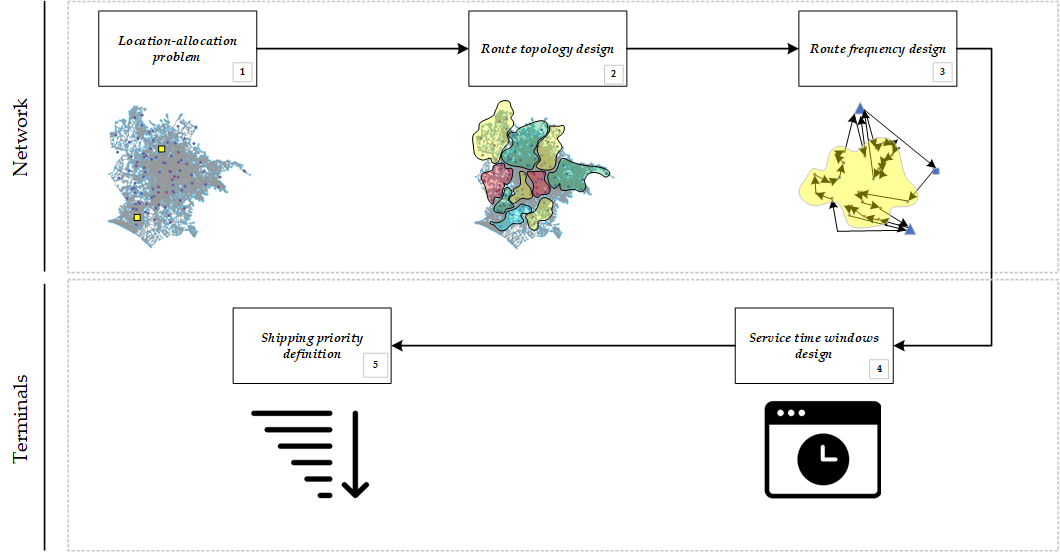
\includegraphics[width=0.9\textwidth]{SectionDistribution/design_figures/fig_network_design.png}
\captionsetup{type=figure}
\caption{Hierarchy of decision problems for distribution network design.}
\label{fig_network_design}
\end{figure}

\section{Location – allocation problem  (P6)}
Location allocation problem (LAP) is a classic operations research problem defined as follows.
Given:
\begin{itemize}
    \item The $n$ nodes of a distribution network;
	\item The requirements for each node;
	\item The shipping cost;
\end{itemize}

Determining:

\begin{enumerate}
    \item A number $m$ of resources to place
	\item Where to place each resource;
	\item The capacity needed by each resource.

\end{enumerate}

The capacity may be the inventory level of a storage system or the throughput of a production plant. The problem definition is general and links together the position on a graph with an amount of capacity. 
\subsection{Model-driven methods (PS3)}
LAP problem requires a model to be solved since it is hard to collect observation on different realisations of a LAP solution. For this reason, we only approach the problem using a model-driven approach. One of the first approaches to the LAP problem sharply identify two main cost function to model and minimise to obtain the optimal solution of the problem ~\cite{Cooper1963}. Let us consider the cost functions:

\begin{equation}
    C^{PLANT}=f(m)
\end{equation}

\begin{equation}
    C^{DIST}=g(m)
\end{equation}

The total cost to minimise is given by $E=C^{PLANT}+C^{DIST}$ where:

\begin{itemize}
    \item $C^{PLANT}$ represents the cost connected to opening a number of resources $m$ (e.g. the cost of the land, the building, the depreciation, the energy, the direct labour);
    \item $C^{DIST}$ represents the cost connected to serving the n nodes of the network using the $m$ selected facilities (e.g. the cost of distribution).
\end{itemize}

From this perspective, the LAP problem represents a generalisation of the facility location problem introduced in section \ref{secFacilityLocationProd} where the optimal facility location is the coordinate where $C^{DIST}$ has a minimum.\par
From a mathematical perspective, the optimal solution to the LAP problem is given by:
\begin{equation}
    \frac{dE}{dm}=\frac{df(m)}{dm}+\frac{dg(m)}{dm}=0
    \label{eqLAP}
\end{equation}

Solving equation (\ref{eqLAP}) in the variable $m$ provides the optimal solution to the LAP problem. Unluckily, solving equation (\ref{eqLAP}) is computationally expensive, and there is no guarantee on how functions $f$, and $g$ have been defined. They are generally not linear, and hard to estimate. Thinking of moving on their surface (if a continuous surface exists) is science fiction.\par

Nevertheless, in practice, both $C^{PLANT}$, and $C^{DIST}$ are easy and fast to estimate for a finite set of solutions of the LAP. A smart approach is to evaluate the total cost $E_\chi$ for a finite number of scenarios $\chi$. Often these scenarios already exist in the mind of the decision-makers. A comparison between these scenarios immediately leads to the most profitable one.

\subsection{Application}
We show an example of an application of the LAP problem by comparing a network in two alternative scenarios: as-is scenario describing the current situation of the network, and to-be scenario evaluating an alternative. The comparison method evaluates the differential cash flows in the two scenarios in a Montecarlo fashion.\footnote{An example of this application is available \href{https://github.com/aletuf93/logproj/blob/master/examples/DIST_04\%20Location-Allocation\%20problem.ipynb}{here}}  \par

A cost model is defined to identify which cost items are relevant to compare the two scenarios, for example:

\begin{itemize}
    \item the direct labour cost;
    \item the cost of logistics and distribution;
    \item the operating costs (e.g. the energy);
    \item the fixed costs to operate the plant;
    \item the depreciation cost;
    \item the investment cost (only for the to-be scenario).
\end{itemize}

The sum of these cost items (except for the depreciation cost) determined the cash flow in each scenario. The difference between the to-be and the as-is scenario determines the differential cash flow. Extending this analysis to a significant time horizon (e.g. ten years) identify the payback period of the to-be investment. When a probability distribution is given for all the cost items identified above, it is possible to determine the risk of the investment using a Montecarlo simulation. The Montecarlo simulation identifies different behaviour, randomly generating numbers from the distribution of the input cost items. Figure \ref{fig_LAP} illustrates the Montecarlo approach and the static approach applied to sample data. This approach can be used to evaluate multiple LAP alternatives compared to an existent scenario identifying which alternative produce an adequate return on the investment.

% INSERT fig_LAP
\begin{figure}[hbt!]
\centering
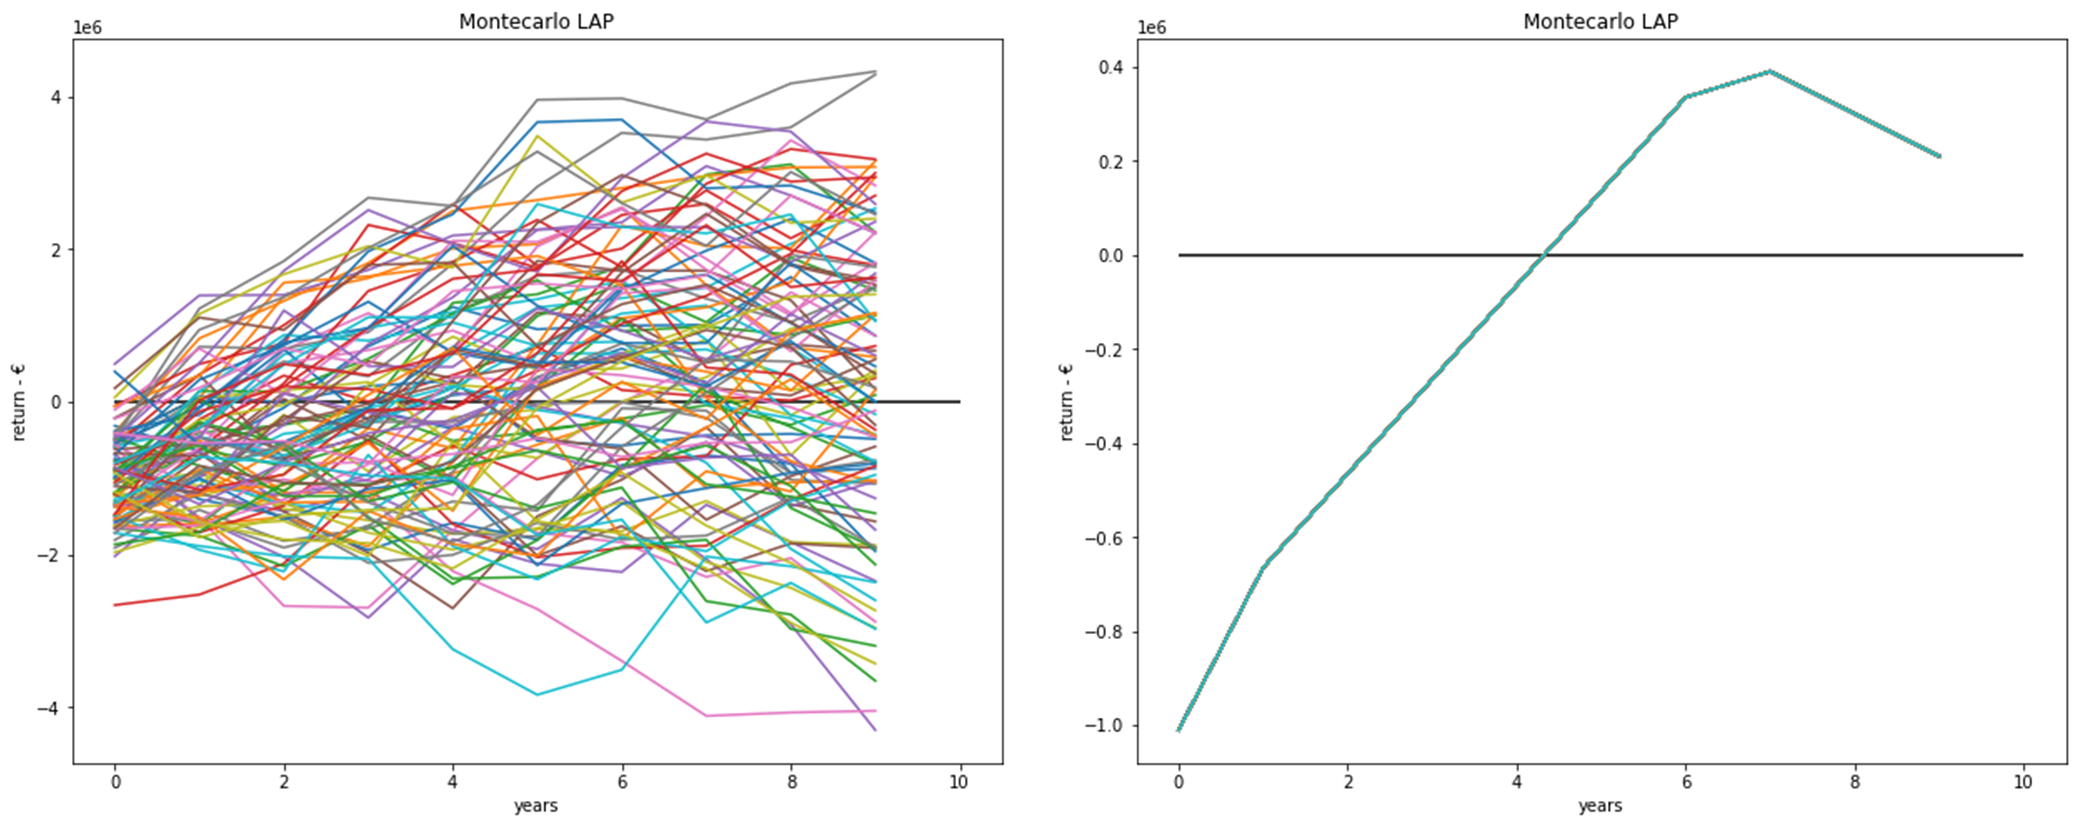
\includegraphics[width=0.9\textwidth]{SectionDistribution/design_figures/fig_LAP.png}
\captionsetup{type=figure}
\caption{Montecarlo and static simulations to evaluate the cash flows of a LAP configuration compared to the existent scenario.}
\label{fig_LAP}
\end{figure}


\section{Network topology design (P2)}
Defining the topology of a network consists of grouping terminals $j$ together, such that a single facility can serve all of them without exceeding its capacity. For example, assigning a distribution centre to a set of points of demand provides a solution to this problem.\par

This problem is similar to the LAP, but it has a different focus. The LAP determines the number, the location, and the capacity of the facilities to open. On the other side, the network topology design assigns terminals to facilities minimising the service cost and without exceeding the capacity of each facility. 

\subsection{Model-driven methods (PS1)}

Operations research provides models for the capacitated facility-location problem to approach the network topology problem. These models can be thought of adaptations of a set covering problem where the terminals $j$ are the points to be covered by the service of the facility. The basic models have the parameters illustrated in Table \ref{tab_routeTopology}.


% INSERT tab_routeTopology
\begin{figure}[hbt!]
\centering
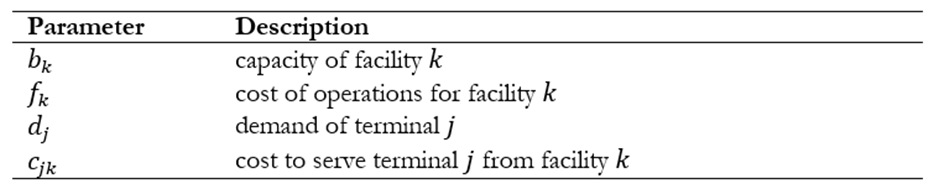
\includegraphics[width=0.9\textwidth]{SectionDistribution/design_figures/tab_routeTopology.png}
\captionsetup{type=table}
\caption{Parameters of the capacitated facility-location problem.}
\label{tab_routeTopology}
\end{figure}

The model has the following variables.

\begin{equation}
   \begin{split}
   y_k=\left\{
                \begin{array}{ll}
                  1\ & if\ facility\ k\ is\ activated\ \\
                  0 & otherwise\\
                \end{array}
              \right.
   \end{split}
\end{equation}

\begin{equation}
   \begin{split}
   x_{jk}=\left\{
                \begin{array}{ll}
                  1 & if\ terminal\ j\ is\ served\ by\ facility\ k\\
                  0 & otherwise\\
                \end{array}
              \right.
   \end{split}
\end{equation}

The problem has the following objective function:

\begin{equation}
    \min{\sum_{k}{f_ky_k+\sum_{j}\sum_{k} c_{jk}}}x_{jk}
\end{equation}

Subjected to the linear constraints:

\begin{equation}
    \sum_{k} x_{jk}=1,\ \forall j
    \label{eqUFLP_1}
\end{equation}

\begin{equation}
    x_{jk}\le y_k,\ \forall j,\forall k
    \label{eqUFLP_2}
\end{equation}

\begin{equation}
    \sum_{j}{d_jx_{jk}\le b_ky_k},\ \forall k
    \label{eqUFLP_3}
\end{equation}

\begin{equation}
    y_k,x_{jk}\in\left\{0,1\right\},\ \forall k,\ \forall j
    \label{eqUFLP_4}
\end{equation}

Constraints (\ref{eqUFLP_1}) impose that all terminal $j$ must be assigned to a facility; constraints (\ref{eqUFLP_2}) links the variables $x$ and $y$; constraints (\ref{eqUFLP_3}) imposes the respect of the capacity of each facility; constraints (\ref{eqUFLP_4}) check the integrality of the decision variables.\par

This model is easy to understand but has many problems in production. The problem is NP-complete, and the number of decision variables $x_{jk}$ is exponential. For these reasons, a branch \& bound algorithm may take forever to solve a real instance of the problem. 

\subsection{Data-driven methods (PS2)}

Data-driven methodologies involve unsupervised learning (see chapter \ref{chapUnsupervisedLearning} that clusters observations into groups given their similarity. Clustering techniques effectively solve the network topology problem since they are computationally efficient. These techniques are uncapacitated. For this reason, we present five approaches to introduce the feasibility check on the capacity parameter. We assume having a number of facilities $m$ with a fixed capacity $C$, equal for all the facilities. All the approaches consider similar input parameters, illustrated in Table \ref{tab_nodeClustering}.

% INSERT tab_nodeClustering
\begin{figure}[hbt!]
\centering
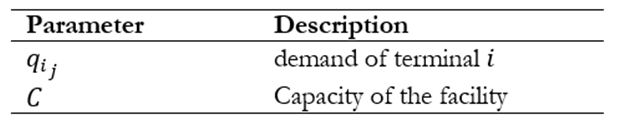
\includegraphics[width=0.7\textwidth]{SectionDistribution/design_figures/tab_nodeClustering.png}
\captionsetup{type=table}
\caption{Parameters of the data-driven methods for the route topology design.}
\label{tab_nodeClustering}
\end{figure}

\subsubsection{Capacitated similarity tree (CST)}
This algorithm builds clusters using a similarity tree produced by hierarchical clustering (see section \ref{secHierarchicalClustering}). Hierarchical clustering aggregates the m observations relying on a proximity matrix $m \times m$, describing how close the observations are. To cluster terminals, we consider a similarity matrix $S$ whose entries $s_{ij}$ measure the closeness of two terminals. $S$ is calculated as the inverse of the matrix of the distances (e.g. the road distance) between nodes. At each step of the algorithm $s_{ij}$ are ordered and the two nodes with the maximum $s_{ij}$ are clustered together if the capacity constraint is respected; otherwise the following $s_{ij}$ is considered for clustering. The algorithm starts creating $m$ clusters. This number is progressively reduced grouping nodes together when the capacity is respected. Algorithm \ref{algo_dist_CST} illustrates the pseudocode for this algorithm.\footnote{The source code of Algorithm \ref{algo_dist_CST} is available \href{https://github.com/aletuf93/logproj/blob/master/logproj/ml_unsupervised_models.py}{here}.} 

\begin{algorithm}[H]
\DontPrintSemicolon
\SetAlgoLined

$i = 1,...,m \in V$ set of vertices\;
$q_i$ demand of vertex $i$\;
$C$ maximum capacity of a cluster \;
$s_{i,j}$ similarity between vertices $i$, and $j$ \;
\For{$k \leftarrow 1:(m-1)$}
{
set $S=\emptyset$\;
$found=false$\;

\While{$not found$}{
$v =\max_{(i,j)-S}{(s_{i,j})}$ \;
$(h,l)=\arg(v)$\;
\eIf{$(q_h+q_l \leq C)$}
    {
    $found=true$ \;
    }
    {
    $S=S \bigcup (h,l)$\;
    }
}
$q_h=q_h+q_l$\;
\For{$r \leftarrow 1: m$}
{
$s_{r,h}=min(s_{r,h},s_{r,l})$\;
$s_{h,r}=min(s_{h,r},s_{l,r})$\;
$s_{r,l}=-1$\;
$s_{l,r}=-1$\;

}
}

\caption{Capacitated similarity tree (CST)}
\label{algo_dist_CST}   
    

\end{algorithm}

\subsubsection{Construction heuristics on a similarity tree (CHST)}
This algorithm works slightly differently from the previous. This algorithm still works on a similarity tree but generating one cluster at a time. When a cluster is full (no residual capacity is left), the algorithm opens a new cluster. A maximum allowable distance $D$ is introduced as a parameter of the algorithm, to avoid that points too “far” enter the same cluster. Algorithm \ref{algo_dist_CHST} illustrates the pseudocode for this algorithm.

\begin{algorithm}[H]
\DontPrintSemicolon
\SetAlgoLined

$i = 1,...,m \in V$ set of vertices\;
$q_i$ demand of vertex $i$\;
$C$ maximum capacity of a cluster \;
$d_{i,j}$ distance between vertices i and j \;
$D$ maximum allowable distance within a cluster \;

$R=V$ \;
$incumbentCluster=false$ \;
\While {($R$ not empty)}{

\If{(not $incumbentCluster$)}
{
$Z= \emptyset$ \;
}

$S= \emptyset $ \;
$v =\min_{(i,j) - S}{(d_{i,j})}$ \;
$(h,l)=\arg(v)$ \;

\eIf{$(q_h+q_l \leq C$ AND $d_{hl} \leq D)$}
    {
    $Z=Z \bigcup (h,l)$ \;
    $R=R - (h,l)$ \;
    \For{$r \leftarrow 1: m$}
{
$s_{r,h}=min(s_{r,h},s_{r,l})$ \;
$s_{h,r}=min(s_{h,r},s_{l,r})$ \;
$s_{r,l}=-1$ \;
$s_{l,r}=-1$ \;

}
    }
    {
    $S=S \bigcup (h,l)$ \;
    \If{$(S==R)$}
    {$incumbentCluster=false$\;}
    }

}


\caption{Construction heuristics on a similarity tree (CHST)}
\label{algo_dist_CHST}       

\end{algorithm}


\subsubsection{Iterative k-means covering algorithm (KCOV)} \label{secKCOV}
This algorithm uses the well-known $k$-means algorithm (see section \ref{secKmeans}) as a generator of columns of a set covering problem (SCP) (see section \ref{secDuality}. The problem us the parameters $c_j$ to identify the cost of a column, and the following variable.

\begin{equation}
   \begin{split}
   x_{j}=\left\{
                \begin{array}{ll}
                  1 & if\ column\ j\ selected \\
                  0 & otherwise\\
                \end{array}
              \right.
   \end{split}
\end{equation}

The problem is defined as follows.

\begin{equation}
    \min{\sum_{j=1}^{n}{x_jc_j}}
\end{equation}

\begin{equation}
    \sum_{j:i\in j}{x_j\geq1} , i\in V
\end{equation}

\begin{equation}
    x_j\in{0;1} , j=1,\ldots,n
\end{equation}

A column $j$ has value '1' at position $i$ if terminal $i$ is included in the cluster; otherwise, its value is '0'. The cost $c_j$ of a column is a measure of saturation and it is calculated at $C-\sum_{i\in j} q_i$. Columns are generated by iteratively running the $k$-means algorithm with increasing values of $k$ (starting from 1 to the number of considered terminals). Only clusters whose capacity falls within a given range are selected as columns of the SCP problem. $k$-means stops increasing when a feasible solution of the SCP exists. The SCP is then optimally solved using branch \& bound algorithm. Algorithm \ref{algo_dist_KCOV} presents the pseudocode of this algorithm.

\begin{algorithm}[H]
\DontPrintSemicolon
\SetAlgoLined
$k=s,...,K =$ neighborhood of the number of centroids \;
$r=$number of replicates\;
$i=1,...,m \in V$ set of vertices \;
$q_i$ demand of vertex $i$ \;
$D_i \in \mathbb{R}^n $ set of coordinates of point i \;
$C$ maximum capacity of a cluster \;
$c$ minimum allowable capacity of a cluster \;
$S= \emptyset $ \;
\For{$k=1:m$}{
    \For{$j=1:r$}{
         $s= $ solution of K-means(k)\;
        \For{cluster $g  \in s$}{
            
            $cap=\sum_{i \in g}^{}{q_i}$\;
                \If{$c \leq cap \leq C$}{
                $S=S \bigcup s$\;
             }
        }
        
    }
}

    
\caption{Iterative $k$-means covering algorithm (KCOV)}
\label{algo_dist_KCOV}    
\end{algorithm}

\subsubsection{Variable neighbourhood search K-means covering algorithm (VKCOV)}

This algorithm works as the previous with a pre-selection on the value of $k$ (i.e. the number of clusters created by the k-means algorithm). All the values of $k$ (i.e., from 1 to the number of terminals) are tested, and it chooses the values of $k$ generating the highest fraction (e.g. the 95\%) of feasible columns (respect with the capacity constraints). Algorithm \ref{algo_dist_VKCOV} illustrates the pseudocode of this algorithm.

\begin{algorithm}[H]
\DontPrintSemicolon
\SetAlgoLined

$k=s,...,K =$ neighborhood of the number of centroids \;
$r=$number of replicates\;
$i=1,...,m \in V$ set of vertices \;
$q_i$ demand of vertex $i$ \;
$D_i \in \mathbb{R}^n $ set of coordinates of point i \;
$C$ maximum capacity of a cluster \;
$c$ minimum allowable capacity of a cluster \;
$S= \emptyset $ \;
\For{$k=1:m$}{
    \For{$j=1:r$}{
         $s= $ solution of K-means(k)\;
         \For{cluster $g  \in s$}{
        
            
            $cap=\sum_{i \in g}^{}{q_i}$\;
                \If{$c \leq cap \leq C$}{
                $S=S \bigcup s$\;
             }
        }
        
    }
}

$\delta = $ select $k \in s,...K$ generating 95 percentile of feasible solutions\;
 
$S= \emptyset $ \;
\For{$k \in \delta$}{
    \For{$j=1:r$}{
        $s= $ solution of K-means(k)\;
        \For{cluster $g  \in s$}{
            
            $cap=\sum_{i \in g}^{}{q_i}$\;
                \If{$c \leq cap \leq C$}{
                $S=S \bigcup s$\;
             }
        }
        
    }
}

\caption{Variable neighbourhood search $k$-means covering algorithm (VKCOV)}
\label{algo_dist_VKCOV}    

\end{algorithm}

\subsubsection{Optimal column generation heuristics (CG)}
This algorithm uses an optimal approach to generate the columns of the SCP presented in paragraph \ref{secKCOV}. The columns are generated while they provide a benefit (i.e. a reduced cost) of the objective function, identifying the closeness of the points within the clusters. A column is generated if:

\begin{itemize}
    \item It has a positive profit;
    \item It respects the capacity constraints;
    \item It respects a distance constraint on the maximum distance of each arc.
\end{itemize}

The primal model of the column generation problem is defined as follows. Table \ref{tab_CG_dist} illustrates the parameters of the problem.

% INSERT tab_CG_dist
\begin{figure}[hbt!]
\centering
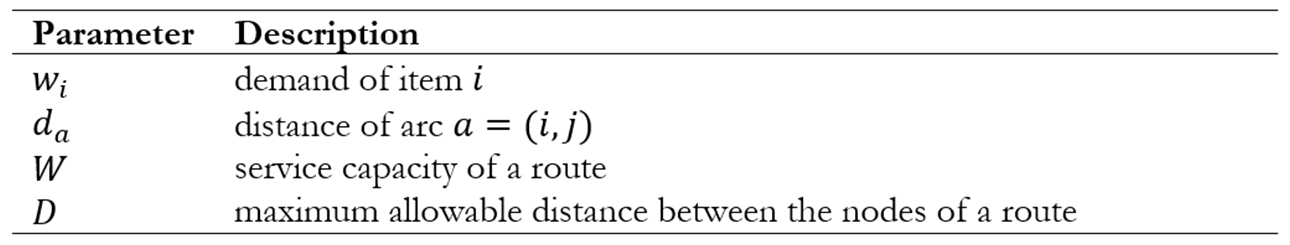
\includegraphics[width=0.7\textwidth]{SectionDistribution/design_figures/tab_CG_dist.png}
\captionsetup{type=table}
\caption{Parameters of primal problem.}
\label{tab_CG_dist}
\end{figure}

The set of the columns of the primal problem is
\begin{equation}
    S=\left\{s\subseteq\left\{i=1,\ldots m\right\}:\sum_{i\in s}{w_i\le W},\ {MAX_{a:i,j\in s}{d}_a\le\ D}\ \right\}
\end{equation}
where $c_s$ is the cost of serving the set $s$. The primal problem has the following variable.

\begin{equation}
   \begin{split}
   x_{s}=\left\{
                \begin{array}{ll}
                  1 & if\ configuration\ s\ is\ selected \\
                  0 & otherwise\\
                \end{array}
              \right.
   \end{split}
\end{equation}

The model is defined as follows.
\begin{equation}
    min\ {c_sx}_S
\end{equation}

\begin{equation}
    \sum_{s\in S:i\in s}{x_s\geq1} , \forall\ i=1,\ldots,m\ 
\end{equation}

\begin{equation}
    x_s\in\left\{0,1\right\} 
\end{equation}

The dual problem is defined as follows.
\begin{equation}
    \max{\pi_i}
\end{equation}

\begin{equation}
    \sum_{i\in S}{\pi_i\le c_s\ , \forall\ s\in S }
\end{equation}

\begin{equation}
    \pi_i\geq0
\end{equation}

The column generation problem find violated dual constraints by solving an optimisation column generation problem with variable

\begin{equation}
   \begin{split}
   \mu_{i}=\left\{
                \begin{array}{ll}
                  1 & if\ i\ belongs\ to\ column\\
                  0 & otherwise\\
                \end{array}
              \right.
   \end{split}
\end{equation}

The model is defined as follows.

\begin{equation}
    \max{\sum_{i=1}^{m}{\mu_i(\pi_i-c_i)}}
\end{equation}

\begin{equation}
    \sum_{i=1}^{m}{\pi_iw_i\le W}
\end{equation}
\begin{equation}
    \mu_i\geq\ z_a , \forall\ \ a=(i,j)
\end{equation}
\begin{equation}
    \mu_j\le z_a , \forall\ \ a=\left(i,j\right)
\end{equation}
\begin{equation}
    \mu_i+\mu_j-1\le z_a , \forall\ \ a=(i,j)
\end{equation}
\begin{equation}
    z_ad_a\le D\ , \forall\ \ a=(i,j)
\end{equation}
\begin{equation}
    \pi_i,z_a\in{0,1}
\end{equation}

\subsection{Application}
We test the five algorithms mentioned above in the field of urban logistics while designing the waste collection service of a wide urban area. The problem involves clustering point of waste production (POWP) together, to assign them to vehicles.\footnote{An example of this application is available \href{https://github.com/aletuf93/logproj/blob/master/examples/DIST_03\%20Route\%20topology\%20design.ipynb}{here}} \par

We define three indicators to evaluate the performance of the algorithm from a computational point of view (see Table \ref{tab_ROMA_application}. The average number of cluster is a measure of the compactness of the outcome clusters. It gives an idea of which algorithm produces, on average, a higher number of classes. It is important to remark that this indicator cannot be directly used as a logistics indicator since it may not be related to the travelled distance within a cluster. The optimal solution of the bin-packing problem (BPP) is calculated, to measure the efficiency of the algorithm in clustering points in the minor number of cluster possible. This solution defines the lower bound of the number of clusters to create. For each algorithm, we measure the gap between its solution and the BPP solution. Besides, we measure the average solving time and the percentage of failing of the algorithms (i.e., the percentage of the instances when an algorithm is not able to find a feasible solution). Since CST and CHST are fully heuristic algorithms, they always provide a feasible solution in a relatively short time.

% INSERT tab_ROMA_application
\begin{figure}[hbt!]
\centering
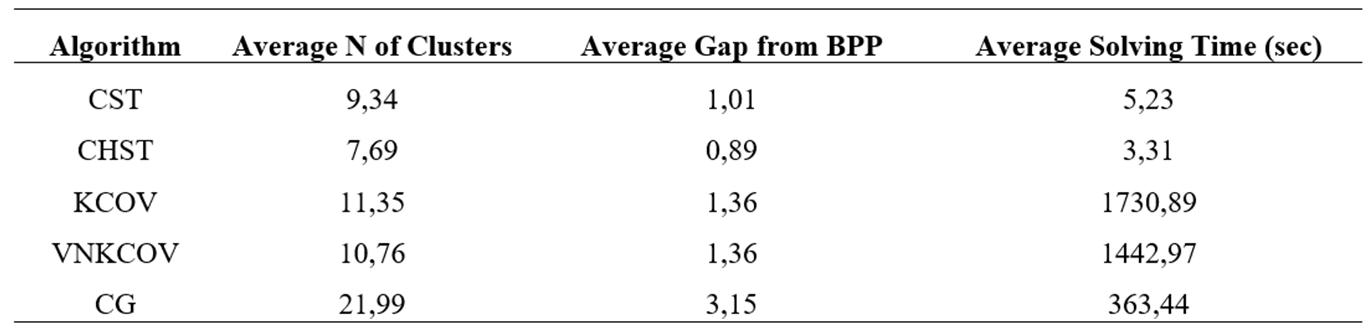
\includegraphics[width=0.9\textwidth]{SectionDistribution/design_figures/tab_ROMA_application.png}
\captionsetup{type=table}
\caption{Performance of the clustering algorithms.}
\label{tab_ROMA_application}
\end{figure}

The logistics performance of each algorithm is evaluated, first, matching the number of clusters (generated by an algorithm)  with the travelled distance (calculated \textit{a posteriori} after solving the TSP problem for each cluster). Figure \ref{fig_ROMA_bolle} presents these analyses showing a dot for each cluster generated by the algorithm in all the 498 instances. The figure shows the number of clusters generated by each algorithm on the $x$-axis of each subplot while the $y$-axis indicates the distance travelled (expressed in km) to serve the POWPs belonging to that cluster. Besides, the colour indicates the number of POWPs in each cluster according to the colour bar. CST and CHST have similar behaviours, but CHST tends to create fewer clusters where more populated clusters account for a higher travelled distance. KCOV and VNKCOV are extremely similar. CG creates clusters whose travelled distance increase with the number of clusters created. Only CG presents a correlation between the number of clusters and the travelled distance. Considering the number of clusters created, the hierarchical algorithms (i.e. CST and CHST) outperform the others since they serve all the nodes with a smaller number of clusters.

% INSERT fig_ROMA_bolle
\begin{figure}[hbt!]
\centering
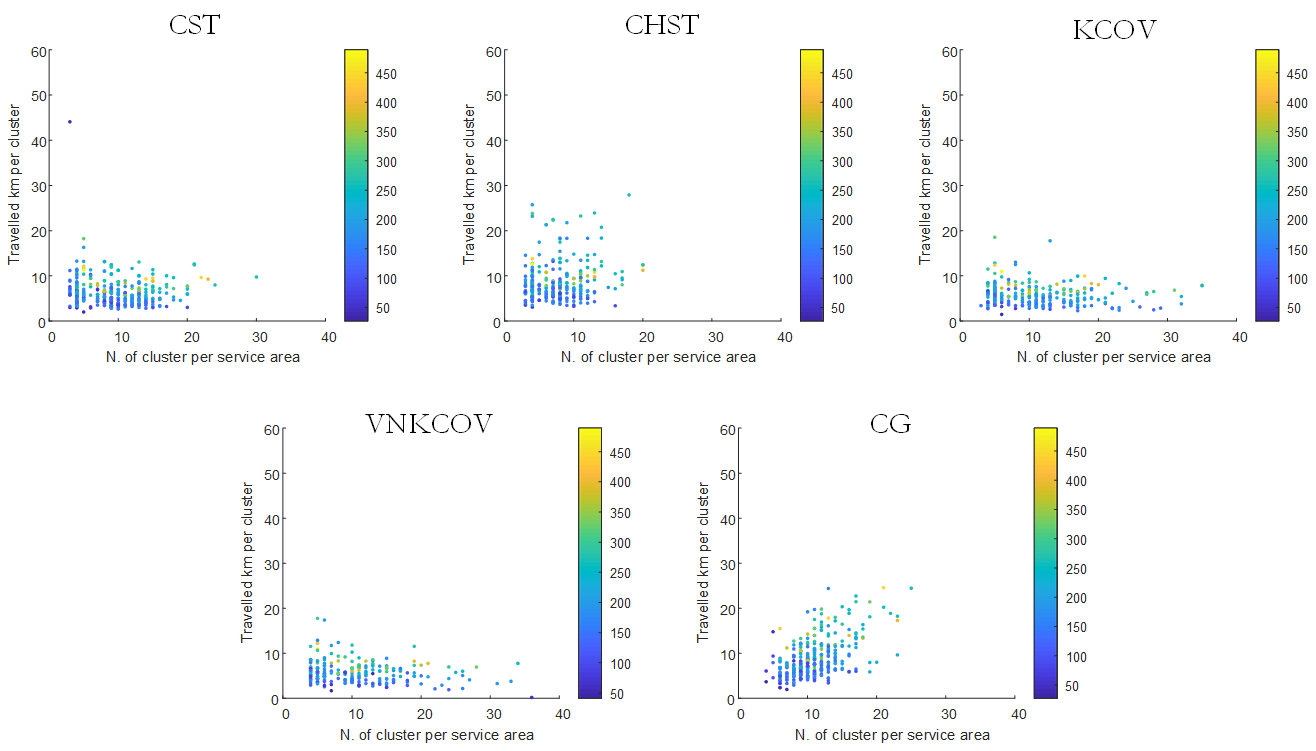
\includegraphics[width=0.9\textwidth]{SectionDistribution/design_figures/fig_ROMA_bolle.png}
\captionsetup{type=figure}
\caption{Scatterplot of the number of cluster per area (x-axis), and travelled km (y-axis).}
\label{fig_ROMA_bolle}
\end{figure}

Figure \ref{fig_ROMA_rette} investigates the correlation between the number of nodes per service area and the travelled distance resulting from the clustering obtained with different algorithms. 

% INSERT fig_ROMA_rette
\begin{figure}[hbt!]
\centering
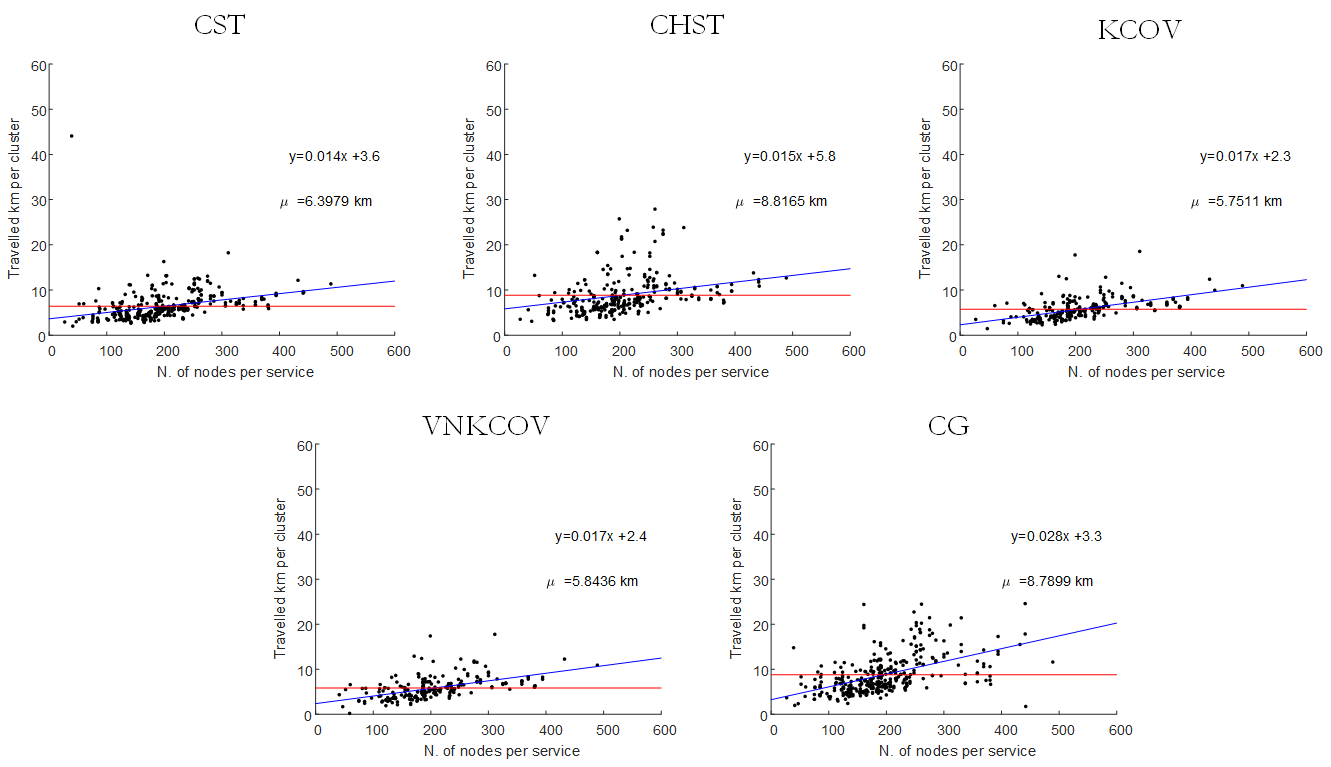
\includegraphics[width=0.9\textwidth]{SectionDistribution/design_figures/fig_ROMA_rette.png}
\captionsetup{type=figure}
\caption{Scatterplot of the number of nodes (x-axis), and km (y-axs) one chart for each algorithm.}
\label{fig_ROMA_rette}
\end{figure}

As the figure shows, in principle, it always exists a correlation between the number of nodes to serve and the distance travelled to connect them. Nevertheless, different algorithms allow obtaining very diverse performance. The performance is measured using the mean value (red line) of the distance travelled to serve each cluster. The blue line identifies the linear regression of the points. CST has a lower average distance value than CHST. Nevertheless KCOV and VNKCOV produce denser clusters with a lower travelled distance. CG, in this case, does not lead to good performance. This can be partly explained thinking at the objective function of the CG algorithm that maximises the saturation of the trucks considering the travelling distance as a constraint (and not as an objective function). \par

Another important logistic indicator is the working time needed to perform a service. This amount of time must match the estimate of time needed to perform operations within each area of service. To get a measure of the feasibility in time of the solution proposed by the algorithms, historical data are considered to assign the time performance to the travelled distance identified by the route design. An average collection speed of 10 km/h is considered and a fixed time of 30 minutes is considered for the operations at the collection points. Given these values, the time effect produced by the algorithms is statically computed. Figure \ref{fig_ROMA_time} presents the histogram of the expected time necessary to serve each area of service with the solution proposed by the clustering algorithms. The feasibility in time of the routes is considered based on the existing working shift of 6 hours. CST and CHST provide a higher percentage of time-feasibility (66,6 and 76,8 respectively). About half of the solutions provided by KCOV, VNKCOV and CG are feasible in time while MDSCOV mainly does not fit the available time of the existing working shifts.

% INSERT fig_ROMA_time
\begin{figure}[hbt!]
\centering
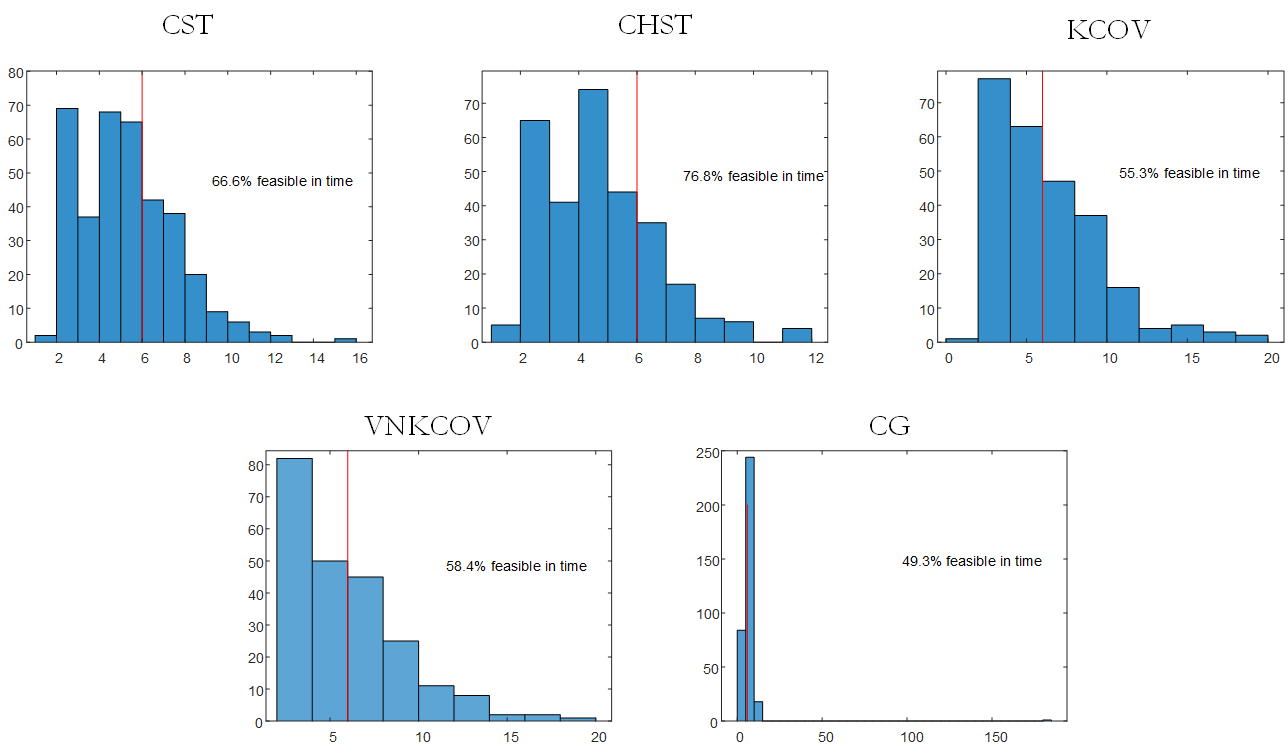
\includegraphics[width=0.9\textwidth]{SectionDistribution/design_figures/fig_ROMA_time.png}
\captionsetup{type=figure}
\caption{Histogram of the estimated service time per area.}
\label{fig_ROMA_time}
\end{figure}

\section{Route frequency design (P5)}
The design of the frequency of a route defines the capacity of the network, and also the saturation of the vehicle. This problem is approached using models to prescribe the power of each route of a network.

\subsection{Model-driven methods (PS4)}
Models to define the frequency of a route can be static or dynamic. When no information about the dynamic behaviour of the demand is available, a static model should be chosen. Static models always work by considering:

\begin{itemize}
    \item $a_v^{e}$, the capacity of the vehicle $v$, serving route $e$;
    \item $b_j$, the demand of a terminal $j$.
\end{itemize}
The minimum frequency of the route $e$, served by a vehicle $v$ can be statically calculated as:

\begin{equation}
    n_j=\left\lceil\frac{b_j}{\sum_{j\in e} a_j}\right\rceil
\end{equation}

When the decision-maker has information on the dynamics of the demand, e.g. its seasonality, a discrete event simulation approach can be preferred to the static approach. Many models adapt real-time the capacity of a route. It is the case of bucket brigades ~\cite{Bartholdi2006}, that adds resources to a route only when these resources are needed.

\section{Service time windows design (P5)}
Time windows design involves the definition of an optimal time horizon to visit all the terminals of a route $e$. Similarly to route frequency, this problem is approached by using models.

\subsection{Model-driven methods (PS4)}
Let consider the problem to define a time windows for a terminal $j$ to be visited by a vehicle $v$ ~\cite{Zuidwijk2017}. We consider a random variable $X$ describing the distribution of arrivals of a vehicle, where $f$ and $F$ are its probability distribution function (PDF) and cumulative distribution function (CDF), respectively. The problem is to identify a time window $\tau\pm\Delta$  when the vehicle is allowed to visit the terminal $j$. A cost of earliness $C^{-}$ is associated with an early arrival (e.g. corresponding to the cost of wait of the vehicle) as well as a cost of tardiness $C^{+}$ is associated with a delay in the arrival (e.g., the waiting cost for the terminal). We assume that the cost of a delay is greater than the cost of early arrival $(C^+>C^-)$, and we introduce $C_r$,  the cost of the terminal resource per unit of time. Figure \ref{fig_time_window} introduces $f(X)$, with the associated costs.

% INSERT fig_time_window
\begin{figure}[hbt!]
\centering
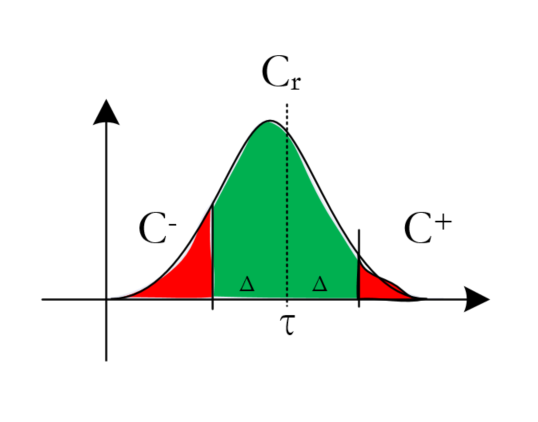
\includegraphics[width=0.9\textwidth]{SectionDistribution/design_figures/fig_time_window.png}
\captionsetup{type=figure}
\caption{Probabilty distribution function of the arrival of a vehicle with the associated costs.}
\label{fig_time_window}
\end{figure}

Based on these parameters, we calculate:
\begin{equation}
    Prob(X<\tau-\Delta)=F(\tau-\Delta)
\end{equation}

\begin{equation}
   Prob(X\geq \tau +\Delta)=1 - F(\tau+\Delta)
\end{equation}

Consequently, three cost items are defined as:
\begin{equation}
   C_{earliness}=C^{-}\times F(\tau-\Delta)
\end{equation}
\begin{equation}
   C_{lateness}=C^{+}\times[1-F(\tau+\Delta)]
\end{equation}
\begin{equation}
   C_{resource}={2C}_r\times \Delta
\end{equation}
\begin{equation}
   C_{tot}=C_{earliness}+C_{lateness}+C_{resource}
\end{equation}

We need to find $\tau$ and $\Delta$ such that $C_{tot}$ is minimised. We introduce the partial derivatives of the cost, and look for the values of $\tau$, and $\Delta$ where the derivatives equal zero.

\begin{equation}
   \begin{split}
   \mu_{i}=\left\{
                \begin{array}{ll}
                  \frac{\partial C_{tot}}{\partial\tau}=0 \\
                  \frac{\partial C_{tot}}{\partial\Delta}=0 \\
                \end{array}
              \right.
   \end{split}
\end{equation}

\begin{equation}
    \frac{\partial C_{tot}}{\partial\tau}=C^{-}\times f(\tau-\Delta)-C^{+}\times f(\tau+\Delta)
    \label{eqPartialDerivativeTau}
\end{equation}

\begin{equation}
    \frac{\partial C_{tot}}{\partial\Delta}= C^{-}\times f(\tau- \Delta)+C^{+} \times f(\tau+\Delta)-2C_r
    \label{eqPartialDerivativeDelta}
\end{equation}

Let assume $X$ being normally distributed: $\frac{1}{\sigma\sqrt{2\pi}}e^\frac{-\left(x-\mu\right)^2}{2\sigma^2}$ . Here it follows the development of the equation (\ref{eqPartialDerivativeTau}).

\begin{equation}
    \begin{split}
        C^{-}\frac{1}{\sigma\sqrt{2\pi}}e^{\frac{-((\tau-\Delta)-\mu)^2}{2\sigma^2}}=
        C^{+}\frac{1}{\sigma\sqrt{2\pi}}e^{\frac{-((\tau+\Delta)-\mu)^2}{2\sigma^2}}\\
        \frac{C^{-}}{C^{+}}e^{\frac{-((\tau-\Delta)-\mu)^2}{2\sigma^2}}=e^{\frac{-((\tau+\Delta)-\mu)^2}{2\sigma^2}}\\
        \log{\left(\frac{C^{-}}{C^{+}}e^{\frac{-((\tau-\Delta)-\mu)^2}{2\sigma^2}}\right)}=\log{\left(e^{\frac{-((\tau+\Delta)-\mu)^2}{2\sigma^2}}\right)}\\
        \log{\left( \frac{C^-}{C^+} \right)} + \log{\left(\frac{C^{-}}{C^{+}}e^{\frac{-((\tau-\Delta)-\mu)^2}{2\sigma^2}}\right)} = \frac{-((\tau + \Delta)-\mu)^2}{2\sigma^2}\\
        \log{\left( \frac{C^-}{C^+} \right)} + \frac{-((\tau - \Delta)-\mu)^2}{2\sigma^2} = \frac{-((\tau + \Delta)-\mu)^2}{2\sigma^2}\\
        2\sigma^2\ln{\left(\frac{C^-}{C^+}\right)} - \left[(\tau - \Delta)^2 + \mu^2 -2\mu(\tau - \Delta)\right] = \\ \left[(\tau + \Delta)^2 + \mu^2 -2\mu(\tau + \Delta)\right]\\
        2\sigma^2\ln{\left(\frac{C^-}{C^+}\right)} - \left[ \tau^2 + \Delta^2 - 2\Delta\tau + \mu^2 -2\mu(\tau - \Delta \right] = \\ \left[ \tau^2 + \Delta^2 + 2\Delta\tau + \mu^2 -2\mu(\tau + \Delta)\right]\\
         2\sigma^2\ln{\left(\frac{C^-}{C^+}\right)} + 2\Delta\tau + 2\mu(\tau - \Delta) = -2\Delta\tau + 2\mu(\tau + \Delta)\\
          2\sigma^2\ln{\left(\frac{C^-}{C^+}\right)} = -4\Delta\tau - 2\mu\tau + 2\mu\Delta + 2\mu\tau + 2\mu\Delta\\
          2\sigma^2\ln{\left(\frac{C^-}{C^+}\right)} = -4\Delta\tau + 4\mu\Delta\\
          \frac{\sigma^2}{2}\ln{\left(\frac{C^-}{C^+}\right)} = \Delta(\mu-\tau)\\
    \end{split}
\end{equation}

For practical reason, the additional variable $u=\frac{\sigma^2}{2}\ln{\left(\frac{C^-}{C^+}\right)}$ is considered, such that:

\begin{equation}
    u=\Delta(\mu-\tau)
    \label{eqTWu}
\end{equation}

Equation (\ref{eqTWu}) is now used to solve the equation (\ref{eqPartialDerivativeDelta}). Please note that from the definition, the term $u$ is a parameter (i.e., it is not function of the variables $\tau$ and $\Delta$). Here it follows the development of the equation (\ref{eqPartialDerivativeDelta}).

\begin{equation}
    \begin{split}
        C^-\times f(\tau-\Delta)+C^+ \times f(\tau+\Delta)-2C_r \\= C^{-}\frac{1}{\sigma\sqrt{2\pi}}e^{\frac{-((\tau-\Delta)-\mu)^2}{2\sigma^2}} + C^{+}\frac{1}{\sigma\sqrt{2\pi}}e^{\frac{-((\tau+\Delta)-\mu)^2}{2\sigma^2}} - 2C_r\\
        C^{-}e^{\frac{-((\tau-\Delta)-\mu)^2}{2\sigma^2}} + C^{+}e^{\frac{-((\tau+\Delta)-\mu)^2}{2\sigma^2}} = 2C_r\sigma\sqrt{2\pi} = \star \\
        C^{-}e^{\frac{-[(\tau-\Delta)^2-\mu^2 -2\mu(\tau-\Delta)]}{2\sigma^2}} + C^{+}e^{\frac{-[(\tau+\Delta)^2-\mu^2 -2\mu(\tau+\Delta)]}{2\sigma^2}} = \star\\
        C^{-}e^{\frac{-[\tau^2+\Delta^2-2\tau\Delta +\mu^2 -2\mu\tau\Delta + 2\mu\Delta]}{2\sigma^2}} + C^{+}e^{\frac{-[\tau^2+\Delta^2+2\tau\Delta +\mu^2 -2\mu\tau\Delta - 2\mu\Delta]}{2\sigma^2}} = \star\\
    \end{split}
\end{equation}

Let be $h=\tau^2+\Delta^2+\mu^2-2\mu\tau$

\begin{equation}
    \begin{split}
         C^{-}e^{\frac{-[h-2\tau\Delta+2\mu\Delta]}{2\sigma^2}} + 
         C^{+}e^{\frac{-[h+2\tau\Delta-2\mu\Delta]}{2\sigma^2}}= \star\\
         C^{-}e^{\frac{-[h+2\Delta(\mu-\tau)]}{2\sigma^2}} + 
         C^{+}e^{\frac{-[h-2\Delta(\mu-\tau)]}{2\sigma^2}} =\star\\
         C^{-}e^{\frac{-[h+2u]}{2\sigma^2}} +
         C^{+}e^{\frac{-[h-2u]}{2\sigma^2}} = \star\\
         C^{-}e^{\frac{-[h+2u]}{2\sigma^2}} +
         C^{+}e^{\frac{-[h+2u-4u]}{2\sigma^2}} = \star\\
         C^{-}e^{\frac{-[h+2u]}{2\sigma^2}} +
         C^{+}e^{\frac{-[h+2u]}{2\sigma^2}} e^{\frac{4u}{2\sigma^2}} =
         \star \\
         e^{\frac{-[h+2u]}{2\sigma^2}} \left\{ C^-\ +C^+e^\frac{4u}{2\sigma^2} \right\} = 2C_r\sigma\sqrt{2\pi}\\
         e^{\frac{-[h+2u]}{2\sigma^2}} = \frac{2C_r\sigma\sqrt{2\pi}}{C^-\ +C^+e^\frac{4u}{2\sigma^2}}\\
         \frac{-[h+2u]}{2\sigma^2} = \log{\left( \frac{2C_r\sigma\sqrt{2\pi}}{C^-\ +C^+e^\frac{4u}{2\sigma^2}} \right)}\\
         h=-2\sigma^2\log{\left(\frac{2C_r\sigma\sqrt{2\pi}}{C^-\ +C^+e^\frac{4u}{2\sigma^2}}\right)}-2u \\
         \tau^2+ \Delta^2+\mu^2-2\mu\tau = -2\sigma^2\ln{\left(\frac{2C_r\sigma\sqrt{2\pi}}{C^-\ +C^+e^\frac{4u}{2\sigma^2}}\right)}-2u\\
         \Delta^2 + \tau^2 + \mu^2 -2\mu\tau= -2\sigma^2\ln{\left(\frac{2C_r\sigma\sqrt{2\pi}}{C^-\ +C^+e^\frac{4u}{2\sigma^2}}\right)}-2u\\
         \Delta^2 + (\mu-\tau)^2 = -2\sigma^2\ln{\left(\frac{2C_r\sigma\sqrt{2\pi}}{C^-\ +C^+e^\frac{4u}{2\sigma^2}}\right)}-2u\\
         \Delta^2 +\frac{u^2}{\Delta^2} = -2\sigma^2\ln{\left(\frac{2C_r\sigma\sqrt{2\pi}}{C^-\ +C^+e^\frac{4u}{2\sigma^2}}\right)}-2u \\
         \Delta^4 - \Delta^2 \left(-2\sigma^2\ln{\left(\frac{2C_r\sigma\sqrt{2\pi}}{C^-\ +C^+e^\frac{4u}{2\sigma^2}}\right)}-2u\right) = -u^2\\
         \Delta^2\left( \Delta^2 + 2\sigma^2\log{\left(\frac{2C_r\sigma\sqrt{2\pi}}{C^-\ +C^+e^\frac{4u}{2\sigma^2}}\right)}+2u \right) = -u^2\\
    \end{split}
\end{equation}

The equation admits up to four solutions. But the equation $\Delta^2=-u^2$ is discarded since the solution belongs to the imaginary space. The remaining solutions are given by the followings.

\begin{equation}
    \Delta^2 = -u^2-2\sigma^2\ln{\left(\frac{2C_r\sigma\sqrt{2\pi}}{C^-\ +C^+e^\frac{4u}{2\sigma^2}}\right)}-2u
\end{equation}

\begin{equation}
    \Delta = \pm\sqrt{-u^2-2\sigma^2\ln{\left(\frac{2C_r\sigma\sqrt{2\pi}}{C^-\ +C^+e^\frac{4u}{2\sigma^2}}\right)}-2u}
\end{equation}

Only the positive value of $\Delta$ is taken into account. Finally, considering that:

\begin{equation}
    u=\frac{\sigma^2}{2}\ln{\left(\frac{C^-}{C^+}\right)}
\end{equation}

The optimal values for $\tau$, and $\Delta$ are obtained as

\begin{equation}
    \Delta = \sqrt{-u^2-2\sigma^2\ln{\left(\frac{2C_r\sigma\sqrt{2\pi}}{C^-\ +C^+e^\frac{4u}{2\sigma^2}}\right)}-2u}
\end{equation}

\begin{equation}
    \tau = \frac{\Delta\mu - u}{\Delta}
\end{equation}

We apply these results using an academic proof of concept. Let consider $X$, being normally distributed with parameters $X\sim N\left(60,\sigma\right)$ and $C^+=5$; $C^-=4$; $C_r=0.3$. We may vary the value of $\sigma$ to perform a sensitivity analysis on the results. Figure \ref{fig_tw_example} illustrates the results of the simulation. The first box shows the shape of $f$, varying the value of $\sigma$. The other boxes illustrate the values of $\tau$, $\Delta$, and the total cost. Realistic values exist until $\sigma$ has real value. Imaginary values are plotted with value '-1'. The example shows that the cost increases while the uncertainty (i.e. $\sigma$) increases. The value of $\tau$ increases when the uncertainty increases since we assume a higher cost of the delay than the cost of earliness. The span of the time window $\Delta$ increases up to a critical value of $\sigma$ where the span of $\Delta$ is large enough that the cost of the terminal resources dedicated to the vehicle equals the cost of lateness plus the cost of tardiness.


% INSERT fig_tw_example
\begin{figure}[hbt!]
\centering
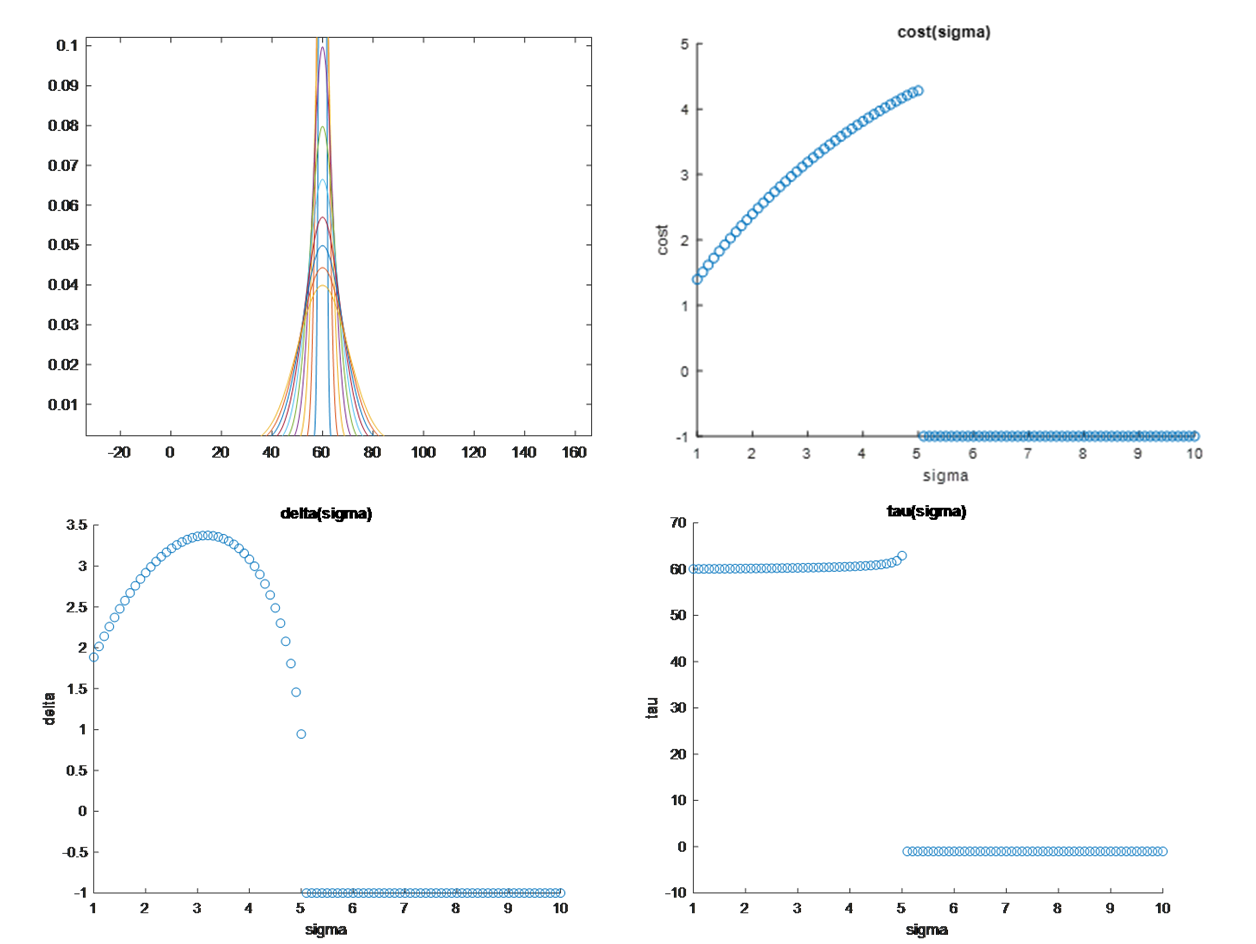
\includegraphics[width=0.9\textwidth]{SectionDistribution/design_figures/fig_tw_example.png}
\captionsetup{type=figure}
\caption{Results of the optimal time windows design.}
\label{fig_tw_example}
\end{figure}

\section{Shipping priority definition (P7)}
The definition of shipping priority is the rationale to assign HUs to vehicles. Usually, shipping companies associate HUs to vehicles based on a FIFO rationale in a push fashion. As soon as an order is available, as soon it has to be assigned. Shipping priority rules answer the question: may we have some benefit by waiting before assigning a HU to a vehicle. The answer to this question is very firm-dependent and product-dependent.\par

When a product is perishable, it is wise to immediately deliver it to provide the consumer with a higher level of service. When a shipping firm has due date to comply with (e.g. deliver within 24, 48, 72 hours) is it appropriate to organise shipping respect with this due dates. In general, the more a HU can wait, the higher the probability of obtaining a better saturation of the vehicle (e.g. loading last-minute orders), see section \ref{secDataDrivenRouting}.







%\clearpage
\bibliographystyle{ieeetr}
\bibliography{SectionDistribution/design_ref}
	
